\documentclass[10pt, a4paper]{scrartcl}

\usepackage{vorschule}
\usepackage[
	typ=ab,
	fach=Informatik,
	lerngruppe={Q1-LK} ,
	nummer=8,
	module={Symbole,Lizenzen},
	seitenzahlen=keine,
	farbig,
	lizenz=cc-by-nc-sa-4,
]{schule}

\usepackage[
	kuerzel=Ngb,
	reihe={Automaten und formale Sprachen} ,
	version={2021-03-07} ,
]{ngbschule}

\author{J. Neugebauer}
\title{Kellerautomaten}
\date{\Heute}

\setzeAufgabentemplate{ngbnormal}

\usepackage{FLaAL}

\usepackage{qrcode}

\renewcommand{\qrhinweis}[1]{%
	\begin{wrapfigure}[4]{r}{0pt}
		\qrcode[height=1cm]{#1}
	\end{wrapfigure}%
}

\begin{document}
\ReiheTitel

Reguläre Sprachen haben ihre Grenzen. Die Sprache $a^nb^n, n\geq 0$ kann nicht durch einen endlichen Automaten akzeptiert werden und wir können auch keine reguläre Grammatik konstruieren. Die Sprache ist also nicht regulär, sondern \emph{kontextfrei}. Um einen Automaten zu konstruieren, der eine kontextfreie Sprache akzeptiert, müssen wir das Automatenmodell erweitern. 

Das Grundproblem: \emph{Ein endlicher Automat kann nicht zählen!} Er kann sich nicht merken, wie viele $a$ schon gekommen sind, um entsprechend viele $b$ abzuzählen. Wir brauchen also eine Struktur, die uns das Zählen erlaubt und diese finden wir im \emph{Keller}.

\begin{infobox}
Ein \emph{nichtdeterministischer Kellerautomat} (NKA) wird als 7-Tupel $A = (Q, \Sigma, K, \delta, q_0, \#, F)$ definiert:
\begin{itemize}
	\item $Q$ ist die (endliche) Menge von Zuständen des Automaten.
	\item $\Sigma$ ist das Eingabealphabet.
	\item $K$ ist das Kelleralphabet.
	\item $\delta: Q\times (\Sigma\cup \{\varepsilon\}) \times K\rightarrow \mathcal P(Q \times K^{*})$ ist die Übergangsfunktion.
	\item $q_0\in Q$ ist der Startzustand.
	\item $\#\in K$ ist das Startsymbol des Kellers.
	\item $F\subset Q$ ist die Menge der Endzustände.
\end{itemize}
\end{infobox}

\begin{wrapfig}
\begin{wrapfigure}[12]{r}{0pt}
	\centering
	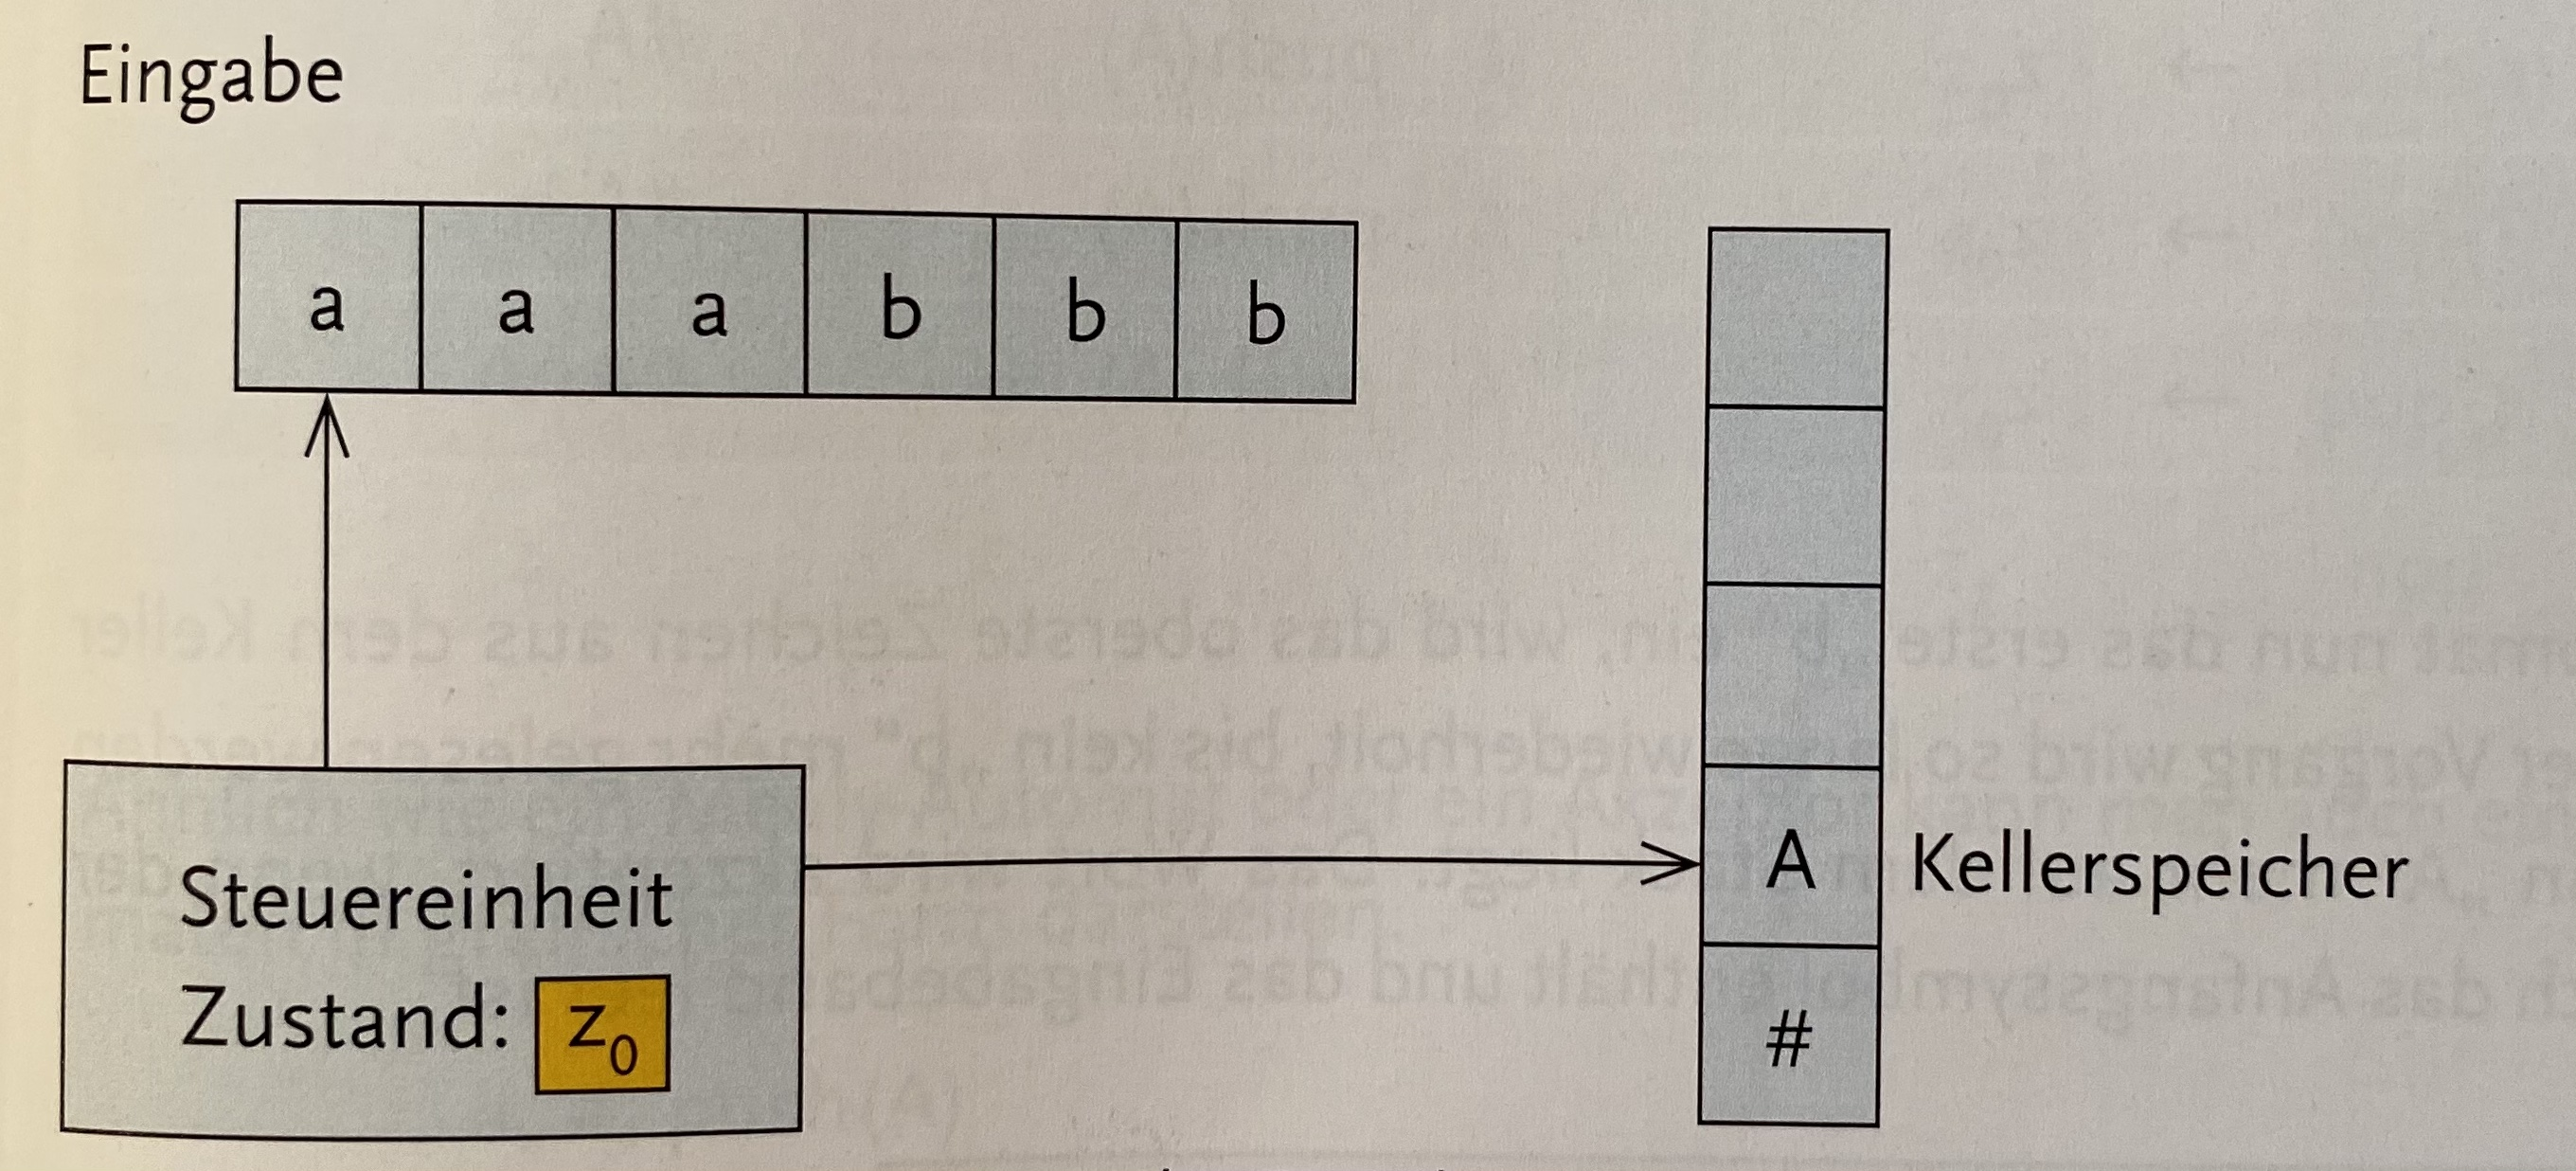
\includegraphics[width=6cm]{Q1-LK-AB.08-Kellerautomaten.jpeg}
	\caption{Schematische Darstellung eines Kellerautomaten}
	\label{abb:schema_nka}
\end{wrapfigure}
Schematisch kann man sich einen Kellerautomaten wie in \prettyref{abb:schema_nka} vorstellen.

Jeder Übergang liest nun nicht mehr nur einen Buchstaben aus dem Eingabealphabet, sondern auch einen Buchstaben aus dem Kelleralphabet: Den obersten Buchstaben auf dem Keller. Das Kellerstartsymbol $\#$ liegt zu Beginn im Keller. Wenn es gelesen wird, dann gilt der Keller als leer.

Zur Darstellung des Übergangsgraphen erweitern wir die Darstellung eine endlichen Automaten um das Kelleralphabet:
\end{wrapfig}

\begin{figure}[h]
	\centering
    \begin{transitiongraph}[pa]
	        \state[s]{q0}{0}{0}
	        \state{q1}{30}{0}
	        \state[f]{q2}{60}{0}
	        \transition{q0}{q0}{\#,a,A\#;A,a,AA}
	        \transition{q0}{q1}{A,b,}
	        \transition{q1}{q1}{A,b,}
	        \transition{q1}{q2}{\#,,}
	    \end{transitiongraph}
	\caption{Kellerautomat zur Sprache $L_K= a^nb^n$ (Klammersprache).}
	\label{abb:nka_klammern}
\end{figure}

Ein Übergang hat nun die Form $(X, Y): Z^{*}$, wobei $X\in K$, $Y\in \Sigma$ und $Z\in K$ sind. Zu beachten ist, dass die Folge von Kellersymbolen $Z^{*}$ von links nach rechts auf den Keller gelegt werden. Für $Z = \varepsilon$ wird nichts auf den Keller gelegt. Da immer das oberste Kellersymbol gelesen wird, wird also ein Buchstabe vom Keller entfernt!

\newpage

\begin{aufgabe}
\label{aufg:nka_klammern}
Baue den Kellerautomaten zur Klammersprache in \prettyref{abb:nka_klammern} in FLACI nach und teste ihn.
\end{aufgabe}

\begin{aufgabe}
\label{aufg:nka_klammern2}
in der Regel ist nicht nur die Verschachtelung von Klammerpaaren ineinander erlaubt, sondern auch mehrere Klammerpaare hintereinander.

Erweitere den Klammerautomaten zur Sprache
\[ L_{K2} = (a^{n_i}b^{n_i})^{m}, n_i\geq 1, m\geq 0, i = 1,...,m \]

Gültige Worte sind zum Beispiel: 
\begin{tasks}(3)
	\task aaabbbaabb
	\task ababab
	\task aabbaabb
\end{tasks}
\end{aufgabe}

\begin{aufgabe}
\label{aufg:nka_gleichlang}
Entwickele in FLACI einen NKA für die Sprachen $L_3$ und $L_4$:

\[ L_3 = \{ w_1 a w_2 | w_1\text{ und }w_2\text{ sind gleichlange Worte über }\{1,0\} \} \]
\[ L_3 = a^nb^m, 0 \leq a <b \]

Gib die formalen Definitionen der Automaten als 7-Tupel an.
\end{aufgabe}

\begin{aufgabe}
\label{aufg:grammatiken_gleichlang}

Erstelle zu den Sprachen $L_3$ und $L_4$ aus \prettyref{aufg:nka_gleichlang} jeweils eine kontextfreie Grammatik, die die Sprachen erzeugt.
\end{aufgabe}

\end{document}